\documentclass{standalone}
\usepackage{tikz}
\begin{document}
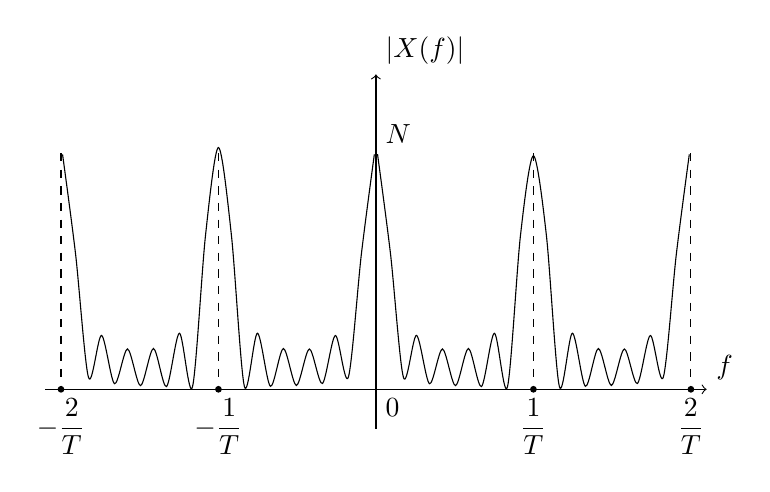
\begin{tikzpicture}[scale=2]
    \draw[->](-2.1,0)--(2.1,0)node[above right]{$f$};
    \draw[->](0,-0.25)--(0,2)node[above right]{$|X(f)|$};
    \node[above right]at(0,1.5){$N$};
    \node[below right]at(0,0){$0$};

    \draw[-]plot[smooth, domain=-1.99:-0.01](\x,{abs((sin(6*pi*\x r))/(4*sin(pi*\x r)))});        
    \draw[-]plot[smooth, domain=0.01:1.99](\x,{abs((sin(6*pi*\x r))/(4*sin(pi*\x r)))});
    \draw[dashed](1,1.5)--(1,0)node[below]{$\displaystyle\frac{1}{T}$};
    \draw[dashed](-1,1.5)--(-1,0)node[below]{$-\displaystyle\frac{1}{T}$};
    \draw[dashed](2,1.5)--(2,0)node[below]{$\displaystyle\frac{2}{T}$};
    \draw[dashed](-2,1.5)--(-2,0)node[below]{$-\displaystyle\frac{2}{T}$};
    \filldraw[black](1,0)circle(0.5pt);
    \filldraw[black](-1,0)circle(0.5pt);
    \filldraw[black](2,0)circle(0.5pt);
    \filldraw[black](-2,0)circle(0.5pt);
\end{tikzpicture}
\end{document}